\let\negmedspace\undefined
\let\negthickspace\undefined
\documentclass[journal]{IEEEtran}
\usepackage[a5paper, margin=10mm, onecolumn]{geometry}
%\usepackage{lmodern} % Ensure lmodern is loaded for pdflatex
\usepackage{tfrupee} % Include tfrupee package

\setlength{\headheight}{1cm} % Set the height of the header box
\setlength{\headsep}{0mm}     % Set the distance between the header box and the top of the text

\usepackage{gvv-book}
\usepackage{hyperref}
\usepackage{gvv}
\usepackage{cite}
\usepackage{amsmath,amssymb,amsfonts,amsthm}
\usepackage{algorithmic}
\usepackage{graphicx}
\usepackage{textcomp}
\usepackage{xcolor}
\usepackage{txfonts}
\usepackage{listings}
\usepackage{enumitem}
\usepackage{mathtools}
\usepackage{gensymb}
\usepackage{comment}
\usepackage[breaklinks=true]{hyperref}
\usepackage{tkz-euclide} 
\usepackage{listings}
% \usepackage{gvv}                                        
\def\inputGnumericTable{}                                 
\usepackage[latin1]{inputenc}                                
\usepackage{color}                                            
\usepackage{array}                                            
\usepackage{longtable}                                       
\usepackage{calc}                                             
\usepackage{multirow}                                         
\usepackage{hhline}                                           
\usepackage{ifthen}                                           
\usepackage{lscape}
\usepackage{circuitikz}
\usepackage{titlesec}
\usepackage{placeins}
\usepackage{pgfplots}
\tikzstyle{block} = [rectangle, draw, fill=blue!20, 
    text width=4em, text centered, rounded corners, minimum height=3em]
\tikzstyle{sum} = [draw, fill=blue!10, circle, minimum size=1cm, node distance=1.5cm]
\tikzstyle{input} = [coordinate]
\tikzstyle{output} = [coordinate]
\titleformat{\section}[hang]{\normalfont\bfseries}{\thesection}{1em}{}
\usepackage{graphicx}
\usepackage{setspace}
\usepackage{hyperref}
\usepackage{xcolor}
\usepackage{tikz}
\usepackage{listings}
\usepackage{xcolor}

\lstset{
  language=python,
  backgroundcolor=\color{black!5},   % light gray background
  basicstyle=\ttfamily\small,         % Monospaced font for code
  breaklines=true,                    % Line wrapping
  keywordstyle=\color{blue},           % Keywords in blue
  commentstyle=\color{green},         % Comments in green
  stringstyle=\color{red},            % Strings in red
  identifierstyle=\color{black},      % Identifiers in black
  emph={def,class}, emphstyle=\bfseries,  % Bold function and class names
  morekeywords={import, as},          % Add extra keywords to be highlighted
  frame=single,                       % Single line frame around the code
  rulecolor=\color{black},            % Frame color
  tabsize=4,                          % Number of spaces per tab
  showstringspaces=false              % Don't underline spaces in strings
}

\usepackage{amsmath}
\usepackage{background}
% Set up the background image
\backgroundsetup{
  scale=0.5,                       % Scale the image
  color=black,                   % Image color (you can change it)
  opacity=0.1,                     % Opacity (1 for full opacity)
  angle=0,                       % Image rotation
  position=current page.center,   % Position at the center of the page
  vshift=-5cm,                    % Vertical shift
  hshift=0cm,                    % Horizontal shift
  contents={
\includegraphics[width=\paperwidth, height=\paperheight]{logo.jpg}}  % Include the image
}

\begin{document}

\begin{titlepage}
    \centering
    {\Huge \bfseries Analysis of RC Circuit Response to a Square Wave Input under Different Time Constant Scenarios

 \par}
    \vspace{1cm}
    
\includegraphics[width=5cm]{IITH.png} 
    \vspace{1cm}
   
    {\Large \bfseries Lab Assignment : 02 \par}
    \vspace{0.5cm}
   
    {\large EE1200: Electrical Circuits Lab \par}
    \vspace{2cm}
   
\begin{tabular}{ll}
    \textbf{Harshil Rathan Y } & \textbf{EE24BTECH11064} \\
    \textbf{Y Akhilesh } & \textbf{EE24BTECH11066} \\
\end{tabular}
\vspace{1cm}
\end{titlepage}
\newpage
\tableofcontents
\newpage

\bibliographystyle{IEEEtran}
\vspace{3cm}

\renewcommand{\thefigure}{\theenumi}
\renewcommand{\thetable}{\theenumi}
\setlength{\intextsep}{10pt} % Space between text and floats


\numberwithin{equation}{enumi}
\numberwithin{figure}{enumi}
\renewcommand{\thetable}{\theenumi}
\section{\textbf{Experiment Objectives}}
The primary objectives of this experiment are as follows
\begin{itemize}
    \item To observe the response of an RC circuit to a square wave input, by applying a square wave input to an RC circuit.
    \item To plot the output and input for a transient response for the first five cycles and a steady-state response.
    \item Use markers from the CRO to get the voltage values and the time period and match the values you see on the CRO with your hand calculations.
    \item To understand the relationship between the time constant ($\tau$)and the period of the square wave $T_{wave}$ -
    $RC==T$, $RC>>T$, $RC<<T$
\end{itemize}
\section{Introduction to RC Circuits}
\begin{itemize}
    \item An RC circuit consists of a resistor (R) and a capacitor (C) connected in series or parallel. 
    \item The time constant determines how quickly the circuit responds to changes in input signals. When subjected to a square wave input, the RC circuit exhibits distinct transient and steady-state behaviors depending on the relationship between the time constant and the input signal's time period (T)
    \item The resistor controls the rate of charge and discharge of the capacitor, creating a time-dependent behavior characterized by the time constant $(\tau = RC)$.
\end{itemize}
\begin{itemize}
    \item The capacitor stores energy in its electric field when a voltage is applied
\end{itemize}
\section{Circuit Diagram}

\begin{figure}[H]
    \centering
    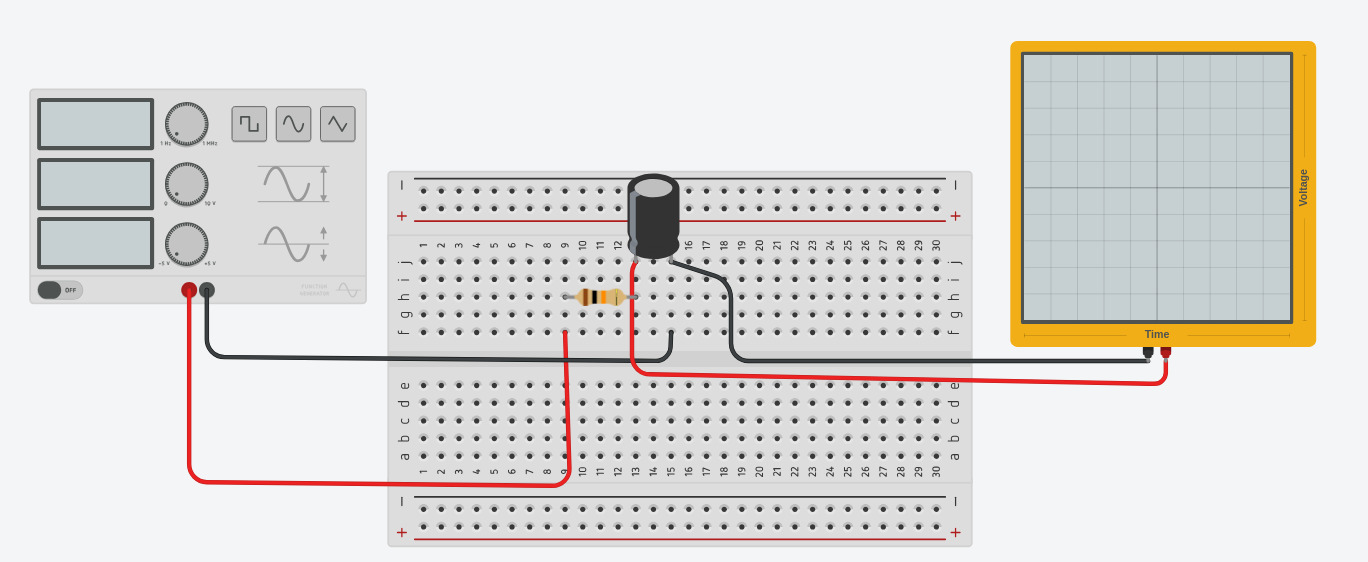
\includegraphics[width=\linewidth]{figs/circuitdiagram.jpeg}
    \label{1}
\end{figure}
Above is the approximate circuit diagram simulated using Tinkercad\\
This circuit diagram represents a simple RC circuit. The key components of the circuit include
\begin{itemize}
    \item Function Generator
    \item Oscilloscope
    \item Breadboard 
    \item Resistor 
    \item Capacitor 
\end{itemize}
\section{Components used }
\subsection{Function Generator}
The function generator serves as the input voltage source for the RC circuit. It provides an alternating signal, typically a square wave, which causes the capacitor to alternately charge and discharge.
\begin{itemize}
    \item Supplies a controlled AC voltage with adjustable frequency and amplitude.
    \item Generates a periodic waveform (such as a square wave) that forces the capacitor to charge and discharge at regular intervals.
    \item Allows experimentation with different signal frequencies to study their effects on the capacitor's behavior.
\end{itemize}
\subsection{Oscilloscope}
The oscilloscope is used to measure and visualize the voltage across the capacitor as it charges and discharges. It provides a real-time graphical representation of how the voltage varies over time.
\begin{itemize}
    \item Captures and displays the capacitor voltage on a time scale, allowing for analysis of the waveform.
    \item Enables measurement of the time constant $\tau$ by determining how long it takes for the capacitor to reach approximately 63% of its final voltage.
\end{itemize}
\subsection{Resistor}
The resistor in the circuit controls the rate at which the capacitor charges and discharges. The value of the resistor along with the capacitor determines the value of the time constant $\tau = RC$, which governs the exponential rate of voltage change across the capacitor.
\begin{itemize}
    \item Limits the current flowing into and out of the capacitor, preventing immediate charging/discharging.
    \item Influences the time constant $\tau$ which affects how fast the capacitor reaches a particular voltage.
\end{itemize}
In this experiment we used a $10k\ohm$ Resistor 
\subsection{Capacitor}
The capacitor is the primary energy storage component in the circuit. It accumulates charge when voltage is applied and releases it when the voltage decreases.
\begin{itemize}
    \item Stores electrical energy when voltage is applied.
    \item Discharges energy when the voltage drops, creating a time-dependent voltage curve.
    \item Demonstrates the principle of exponential charging and discharging.
\end{itemize}
In this experiment we use a $220 \micro F$ capacitor 
\subsection{Breadboard}
The breadboard is used as a platform for assembling the circuit without the need for soldering. It allows for easy modifications and troubleshooting of the circuit.
\begin{itemize}
    \item Ensures proper electrical connections between the function generator, resistor, capacitor, and oscilloscope.
\end{itemize}
\section{Case I : $RC==T$}
In this case the time constant $RC$ matches with the time period of the curve 
\subsection{Diagram}
\begin{center}
    \begin{figure}[!ht]
\centering
\resizebox{0.6\textwidth}{!}{% Adjusted size to fit better
\begin{circuitikz}
\tikzstyle{every node}=[font=\small]

% Main circuit connections
\draw (5,11.5) to[short] (5,9.75); % Vertical connection
\draw (5,11.5) to[short] (7.25,11.5); % Horizontal connection
\draw (7.25,11.5) to[R] (9.25,11.5); % Resistor
\draw (9.25,11.5) to[short] (9.25,10.5); % Vertical to capacitor
\draw (9.25,10.5) to[C] (9.25,8.75); % Capacitor
\draw (5,9.75) to[square voltage source] (5,8); % Voltage source
\draw (5,8) to[short] (9.25,8); % Bottom horizontal connection
\draw (9.25,8.75) to[short] (9.25,8); % Short to ground

% Labels
\node [font=\small] at (4.25,9) {5V}; % Voltage source label
\node [font=\small] at (8.25,12.25) {10k$\ohm$}; % Resistor label
\node [font=\small] at (10.25,9.5) {220$\mu$F}; % Capacitor label

% Output and arrows
\draw (9.25,11.5) to[short] (12.5,11.5); % Horizontal connection from resistor
\draw (9.25,8) to[short] (12.5,8); % Horizontal connection from ground
\node [font=\large] at (12.5,9.5) {V$_c$}; % Label for capacitor voltage
\draw [->, >=Stealth] (12.5,9.75) -- (12.5,11.5); % Arrow to top
\draw [->, >=Stealth] (12.5,9.25) -- (12.5,8); % Arrow to bottom

% Ground symbol
\draw (9.25,8) to (9.25,7.25) node[ground] {}; % Ground connection

% Input voltage label
\node [font=\large] at (5.75,8.75) {V$_{\text{in}}$}; % Label for input voltage

\end{circuitikz}
}%
\end{figure}
\end{center}
\subsection{Input signal}
The input signal is a square wave with a time period \( T = 2.2 \, \text{s} \), alternating between +5V and -5V. 
\begin{figure}[ht]
    \centering
    \begin{tikzpicture}
        \begin{axis}[
            width=10cm, height=6cm,
            grid=major,
            grid style={dashed, gray!30},
            axis lines=middle,
            xlabel={Time (s)},
            ylabel={Voltage (V)},
            xmin=0, xmax=4.4,
            ymin=-5.5, ymax=5.5,
            xtick={0,1,2,3,4},
            ytick={-5, -4, -3, -2, -1, 0, 1, 2, 3, 4, 5},
            every axis x label/.style={at={(current axis.right of origin)}, anchor=north, yshift=-15pt},
            every axis y label/.style={at={(current axis.above origin)}, anchor=east, xshift=-5pt},
            legend pos=south east,
            legend style={draw=none, fill=white, font=\small}
        ]
            % Square wave plot for period 2.2 s
            \addplot[blue, thick] coordinates {
                (0,5) (1.1,5) (1.1,-5) (2.2,-5)
                (2.2,5) (3.3,5) (3.3,-5) (4.4,-5)
            };
        \end{axis}
    \end{tikzpicture}
\end{figure}
\subsection{Input parameters}
\begin{itemize}
    \item $R$ = $10 k \ohm$
    \item $C$ = $220 \mu F$
    \item Square wave input 
        \begin{itemize}
            \item Amplitude = $\pm 5$
            \item Frequency = $0.454545$Hz
            \item Time Period = $2.2s$
        \end{itemize}
\end{itemize}
The value of the time constant in our experiment is $10\times 10^3 \times220 
 \times 10^{-6}$ = $2.2$
\subsection{Observations}
\begin{itemize}
    \item Connect all the components according to the circuit diagram 
    \item Input the signals and parameters mentioned above
    \item First we get a \textbf{periodic(continuous)waveform} and then we fix the number of cycles to get a \textbf{single(captured) waveform}  
\end{itemize}

\subsubsection{Continuous Waveform}
\begin{figure}[H]
    \centering
    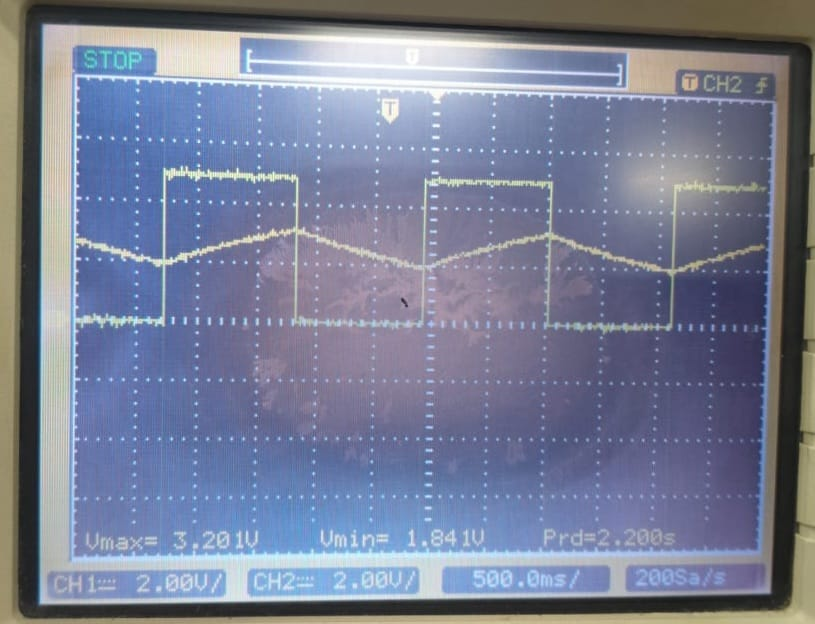
\includegraphics[width=0.75\linewidth]{figs/Rc=t1.jpeg}
\end{figure}
\begin{table}[h]
    \centering
    \renewcommand{\arraystretch}{1.3} % Adjust row height for better readability
    \begin{tabular}{|l|c|}
        \hline
        \textbf{Parameter} & \textbf{Value} \\
        \hline
        Waveform Type & Square Wave \\
        \hline
        Period & 2.200 s \\
        \hline
        Frequency & $\frac{1}{2.2} = 0.4545$ Hz \\
        \hline
        High Level Voltage & 5.000 V \\
        \hline
        Low Level Voltage & 0 mV (0 V) \\
        \hline
        Start Phase & 0° \\
        \hline
    \end{tabular}
\end{table}
The above table are the set of values inputted on the function generator
\subsubsection{Plotting using LTspice}
On simulating the below circuit on LTspice with $T=2.2$s, we can verify the figure that we obtained on the CRO for steady state response 
\begin{center}
    \begin{circuitikz}
\tikzstyle{every node}=[font=\normalsize]
\draw (3.5,10.5) to[short] (3.5,8.25);
\draw (3.5,8.25) to[square voltage source, sources/symbol/rotate=auto] (3.5,7);
\draw (3.5,10.5) to[short] (5,10.5);
\draw (5,10.5) to[R,l={ \normalsize 10k}] (7.75,10.5);
\draw (7.75,10.5) to[C,l={ \normalsize 200$\mu$}] (7.75,6.75);
\draw (3.5,7) to[short] (3.5,6.5);
\draw (3.5,6.5) to[short] (5.5,6.5);
\draw (5.5,6.5) to[short] (7.75,6.5);
\draw (7.75,6.75) to[short] (7.75,7.75);
\draw (7.75,7.75) to[short] (7.75,6.5);
\node [font=\normalsize] at (8,10.75) {$V_c$};
\node [font=\normalsize] at (6.25,10) {$R_1$};
\node [font=\normalsize] at (7,8.75) {$C_1$};
\node [font=\normalsize] at (2.75,7.75) {$V_{in}$};
\end{circuitikz}
\end{center}
\begin{figure}[H]
    \centering
    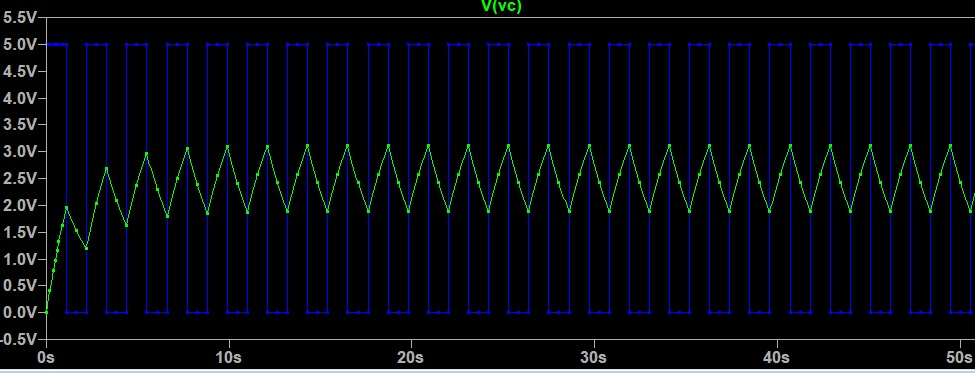
\includegraphics[width=\linewidth]{figs/lt1.jpeg}
\end{figure}
The above figure shows that the circuits eventually attains a steady state response and the values for $V_{max}$, $V_{min}$ obtained also match after approx 10 cycles 
The values obtained according to the simualtion are  
\begin{itemize}
    \item $V_{max} = 3.11V$
    \item $V_{min} = 1.88 V$
\end{itemize}
The values match approximately with the ones on the CRO, there is some error due to noise and other practical factors \\
Hence the plot is verified 
\subsubsection{Verification using Python}
It is difficult to prove the steady state values mathematically hence we use python. Below are code snippets that help verify the steady state value \\
The input variables for the code are given below
\begin{lstlisting}[language=python]
V_high = 5          # High voltage of the square wave (V)
V_low = 0           # Low voltage of the square wave (V)
T = 2.2               # Time period of the square wave (s)
RC = 2.2            # RC time constant (s)
duty_cycle = 0.5    # Duty cycle (50%)
t_high = duty_cycle * T  # Time duration of high phase
t_low = (1 - duty_cycle) * T  # Time duration of low phase
\end{lstlisting}
The below snippet iteratively calculates the steady-state crest and trough voltages of an RC circuit under a square wave input
\begin{lstlisting}[language=python]
while True:
    # Calculate new crest voltage during charging
    V_crest_new = V_high + (V_trough_prev - V_high) * np.exp(-t_high / RC)
    
    # Calculate new trough voltage during discharging
    V_trough_new = V_low + (V_crest_new - V_low) * np.exp(-t_low / RC)
    
    # Check for convergence
    if abs(V_crest_new - V_crest_prev) < tolerance and abs(V_trough_new - V_trough_prev) < tolerance:
        break
    
    # Update previous values for the next iteration
    V_crest_prev = V_crest_new
    V_trough_prev = V_trough_new
\end{lstlisting}
On executing this python code we get the values of $V_{max} = 3.112296$ and $V_{min} = 1.887703$ \\
Which is close to the values obtained on simulation via LTspice and the CRO \\
Hence the steady state response for $RC==T$ is verified 
\subsubsection{Single Waveform}
The single waveform obtained for 5 cycles is below 
\begin{figure}[H]
    \centering
    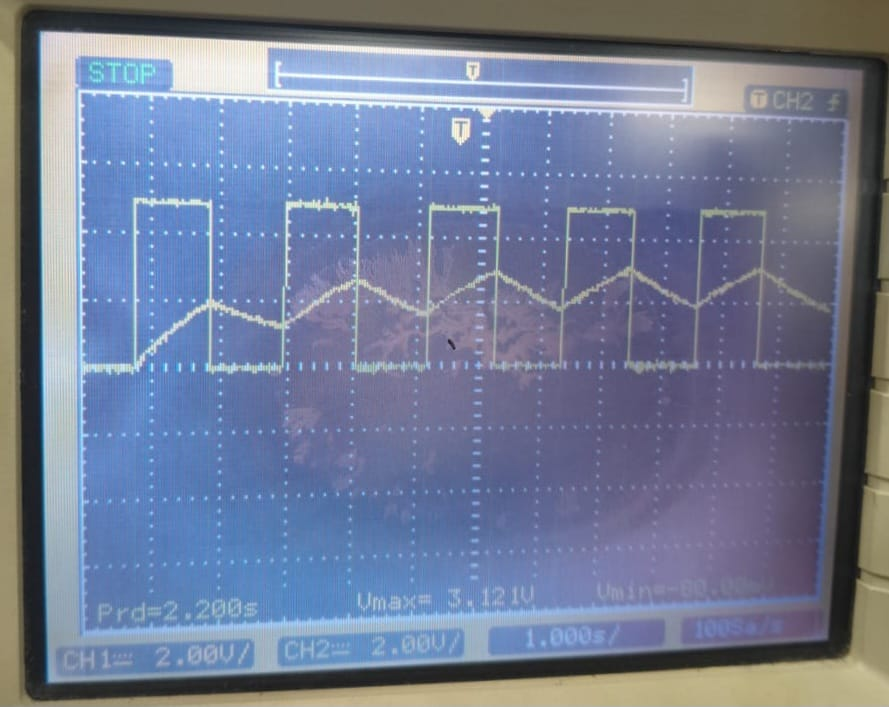
\includegraphics[width=0.8\linewidth]{figs/Rc=t2.jpeg}
\end{figure}
The transient response is obtained for the below parameters, no. of cycles is set to 5 
\begin{figure}[H]
    \centering
    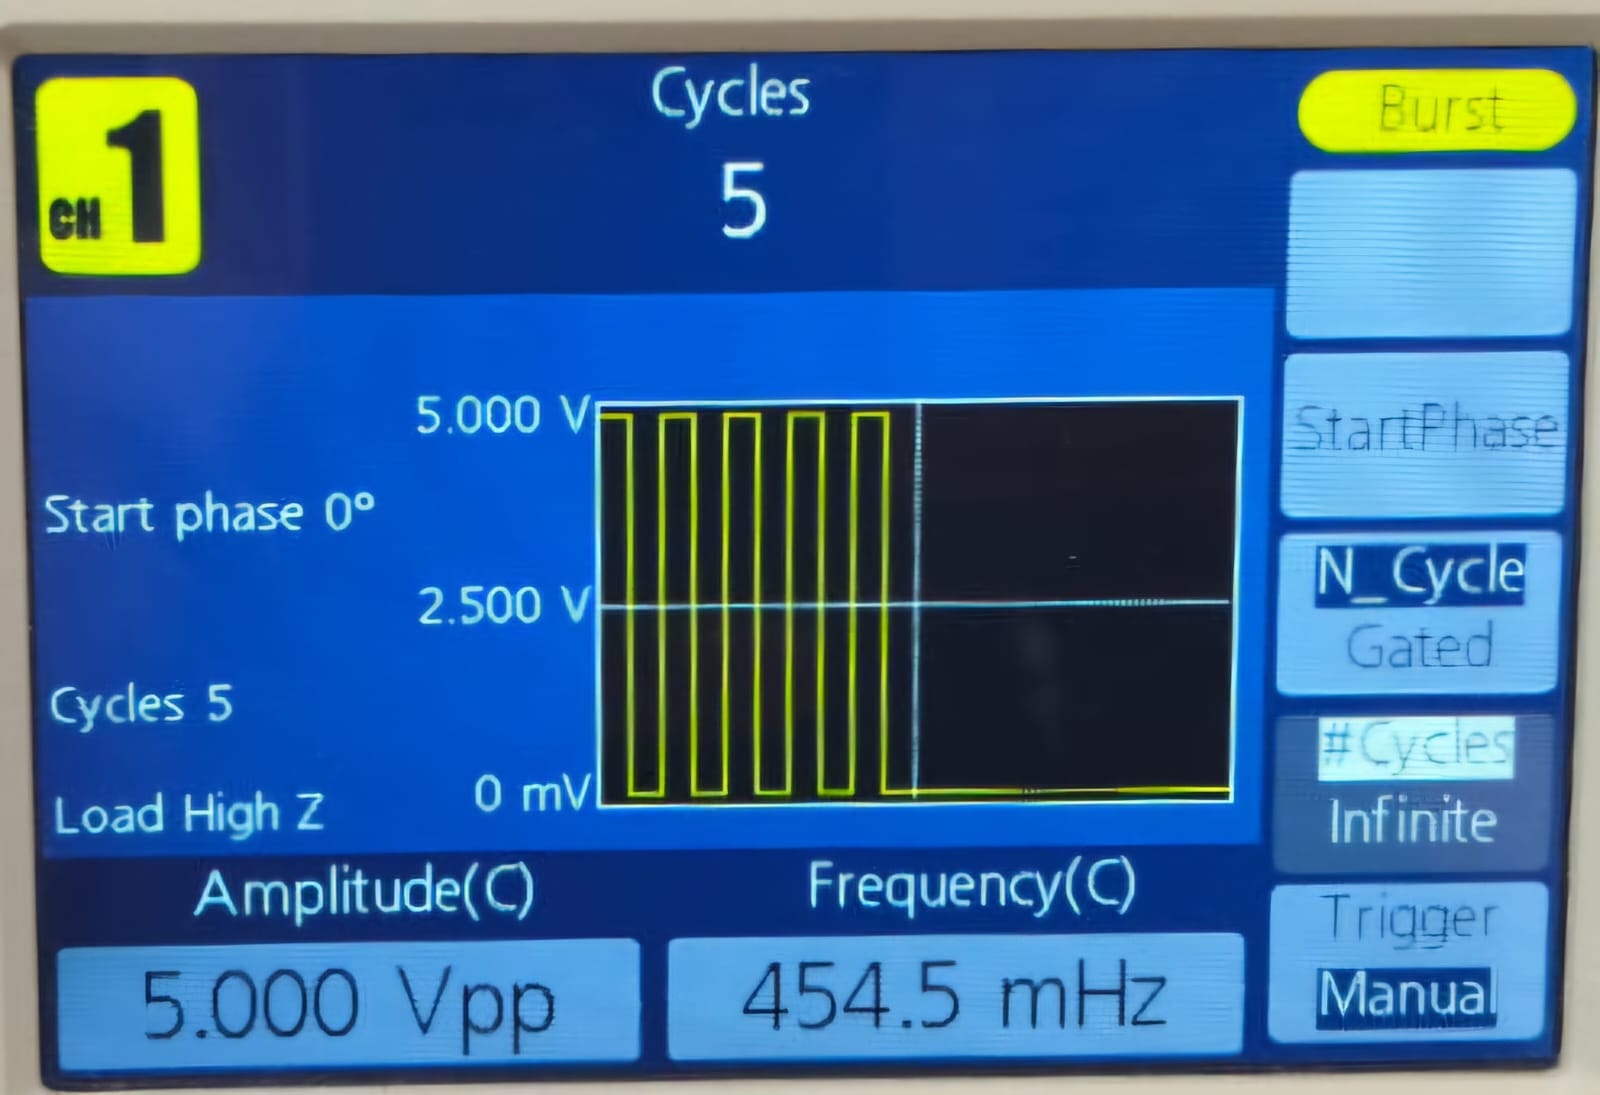
\includegraphics[width=0.5\linewidth]{figs/ip1.jpeg}
\end{figure}
\subsubsection{Mathematical Proof}
During charging of capacitor 
\begin{align*}
    V_c = V_{max}(1-e^{\frac{-t}{\tau}})
\end{align*}
Where t goes from 0 to $\frac{t}{2}$
During discharging of capacitor
\begin{align*}
    V_c = V_{initial}(e^{\frac{-t}{\tau}})
\end{align*}
where $V_{initial}$ = voltage at $\frac{t}{2}$ \\
The RC value for this experiment is 2.2 \\
Time period = 2.2 s
\begin{itemize}
    \item Where the time period is 2.2s, the half-period is
    \begin{align*}
        \frac{T}{2}=1.1
    \end{align*}
\end{itemize}
During the charging phase the voltage across the capacitor is given by 
\begin{align*}
    V_c(\frac{T}{2}) = V_{max}(1-e^{\frac{-T/2}{\tau}}) 
\end{align*}
$\tau=2.2$ and $\frac{T}{2}=1.1$, on substituting 
\begin{align*}
    V_c(\frac{T}{2}) = 5(1-e^{-0.5})
\end{align*}
\begin{align*}
    V_c(\frac{T}{2}) = 5(1-0.6065) 
\end{align*}
\begin{align*}
    V_c(\frac{T}{2}) \approx 1.9675
\end{align*}
The voltage per division is recorded as 2.2 on the CRO which is approximately equal to the value obtained, there is always some error due to noise and other factors \\
During discharge of the capacitor, the capacitor discharges from $V_{initial} = 1.9675$
\begin{align*}
    V_C(T) = V_{initial}(e^{\frac{-T/2}{\tau}})
\end{align*}
\begin{align*}
    V_C(T) = 1.9675(e^{-0.5})
\end{align*}
On substituting we get 
\begin{align*}
    V_C(T) = 1.9675(0.6065) = 1.1932 
\end{align*}
The values of $V_C(T)$ and $V_C(T/2)$ match with the values on the oscilloscope hence the transient state response is proved mathematically 
\subsubsection{Plotting usig LTspice}
\begin{figure}[H]
    \centering
    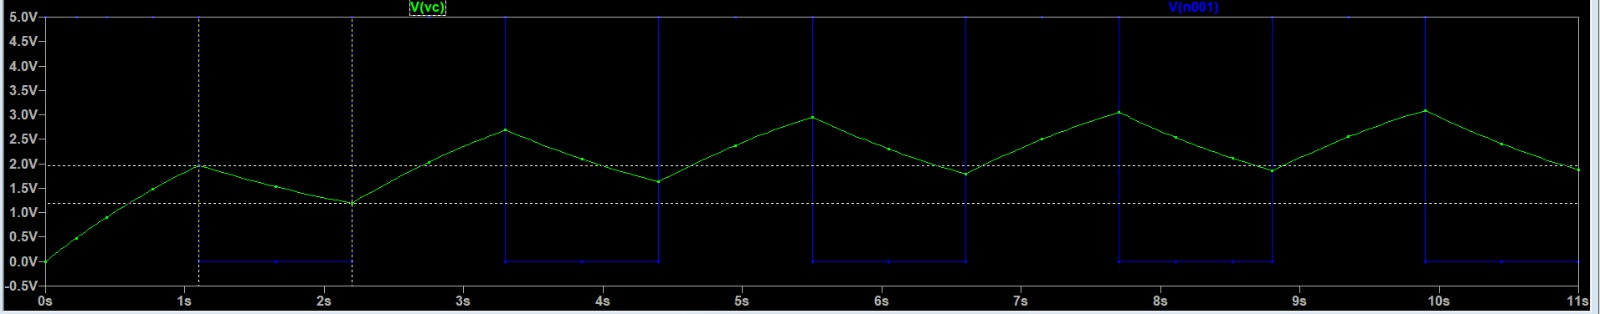
\includegraphics[width=\linewidth]{figs/lt1.2.jpeg}
\end{figure}
\begin{figure}[H]
    \centering
    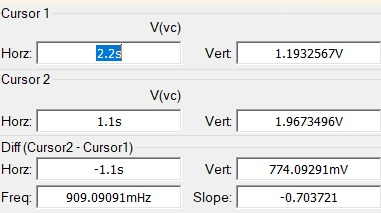
\includegraphics[width=0.7\linewidth]{figs/lt1.3.jpeg}
\end{figure}
As we can see from the figure above, the cursor 1 is placed at T=2.2, $V_C = 1.1932567$ and the cursor 2 is placed at T=1.1, $V_C= 1.9673496$\\
Which is approximately same as the values obtained via mathematical proof \\
Hence the transient response for $RC==T$ for 5 cycles is verified both by simulation and mathematical methods
\section{Case II : \( RC \ll T \)}
In this case, the time constant \( RC \) is much smaller than the time period of the input signal, meaning that the capacitor charges and discharges relatively slowly compared to the input waveform's period. With a time period of \( T = 22 \, \text{s} \), which is much larger than the time constant \( \tau = RC = 2.2 \, \text{s} \), the voltage across the capacitor will have sufficient time to reach a significant portion of the maximum voltage during each cycle.
\subsection{Diagram}
The circuit used for this analysis consists of a resistor and capacitor in series with a square wave input, as shown below:
\vspace{-10pt}
\begin{center}
    \begin{circuitikz}
\tikzstyle{every node}=[font=\small]

% Main circuit connections
\draw (5,11.5) to[short] (5,9.75); % Vertical connection
\draw (5,11.5) to[short] (7.25,11.5); % Horizontal connection
\draw (7.25,11.5) to[R] (9.25,11.5); % Resistor
\draw (9.25,11.5) to[short] (9.25,10.5); % Vertical to capacitor
\draw (9.25,10.5) to[C] (9.25,8.75); % Capacitor
\draw (5,9.75) to[square voltage source] (5,8); % Voltage source
\draw (5,8) to[short] (9.25,8); % Bottom horizontal connection
\draw (9.25,8.75) to[short] (9.25,8); % Short to ground

% Labels
\node [font=\small] at (4.25,9) {5V}; % Voltage source label
\node [font=\small] at (8.25,12.25) {10k$\ohm$}; % Resistor label
\node [font=\small] at (10.25,9.5) {220$\mu$F}; % Capacitor label

% Output and arrows
\draw (9.25,11.5) to[short] (12.5,11.5); % Horizontal connection from resistor
\draw (9.25,8) to[short] (12.5,8); % Horizontal connection from ground
\node [font=\large] at (12.5,9.5) {V$_c$}; % Label for capacitor voltage
\draw [->, >=Stealth] (12.5,9.75) -- (12.5,11.5); % Arrow to top
\draw [->, >=Stealth] (12.5,9.25) -- (12.5,8); % Arrow to bottom

% Ground symbol
\draw (9.25,8) to (9.25,7.25) node[ground] {}; % Ground connection

% Input voltage label
\node [font=\large] at (5.75,8.75) {V$_{\text{in}}$}; % Label for input voltage

\end{circuitikz}
\end{center}

\subsection{Input Signal}

The input signal is a square wave with a time period \( T = 22 \, \text{s} \), alternating between +5V and -5V. 
\begin{figure}[ht]
    \centering
    \begin{tikzpicture}
        \begin{axis}[
            width=10cm, height=6cm,
            grid=major,
            grid style={dashed, gray!30},
            axis lines=middle,
            xlabel={Time (s)},
            ylabel={Voltage (V)},
            xmin=0, xmax=44,
            ymin=-5.5, ymax=5.5,
            xtick={0,10,20,30,40},
            ytick={-5, -4, -3, -2, -1, 0, 1, 2, 3, 4, 5},
            every axis x label/.style={at={(current axis.right of origin)}, anchor=north, yshift=-15pt},
            every axis y label/.style={at={(current axis.above origin)}, anchor=east, xshift=-5pt},
            legend pos=south east,
            legend style={draw=none, fill=white, font=\small}
        ]
            % Square wave plot for period 22 s
            \addplot[blue, thick] coordinates {
                (0,5) (11,5) (11,-5) (22,-5)
                (22,5) (33,5) (33,-5) (44,-5)
            };
        \end{axis}
    \end{tikzpicture}
\end{figure}
\subsection{Input Parameters}

The input signal parameters are summarized in the following table:

\begin{center}
\begin{tabular}{|c|c|}
\hline
\textbf{Parameter} & \textbf{Value} \\
\hline
Resistance \( R \) & \( 10 \, k\Omega \) \\
\hline
Capacitance \( C \) & \( 220 \, \mu F \) \\
\hline
Amplitude of input signal & \( \pm 5 \, V \) \\
\hline
Frequency of input signal & \( \frac{1}{22} \, \text{Hz} \) \\
\hline
Time Period \( T \) & \( 22 \, \text{s} \) \\
\hline
\end{tabular}
\end{center}

The time constant \( \tau \) is calculated as:
\[
\tau = R \cdot C = 10 \times 10^3 \, \Omega \times 220 \times 10^{-6} \, \text{F} = 2.2 \, \text{s}
\]
\subsection{Observations}
\subsubsection{Continuous Waveform}

For the continuous waveform, the input signal repeats indefinitely, maintaining the same characteristics as the square wave. This is shown below.

\begin{figure}[H]
    \centering
    % Place the figure of the continuous waveform here
    \includegraphics[width=\textwidth]{figs/t>>RC-c.jpeg}
\end{figure}
\begin{table}[h]
    \centering
    \renewcommand{\arraystretch}{1.3} % Adjust row height for better readability
    \begin{tabular}{|l|c|}
        \hline
        \textbf{Parameter} & \textbf{Value} \\
        \hline
        High Level Voltage & 5.000 V \\
        \hline
        Low Level Voltage & 0 mV (0 V) \\
        \hline
        Start Phase & 0° \\
        \hline
    \end{tabular}
\end{table}
The above table and the parameters mentioned are the set of values inputted on the function generator
\subsubsection{Plotting using LTspice}
On simulating the below circuit on LTspice with $T=22$s, we can verify the figure that we obtained on the CRO for steady state response \\

Since the time period \( T = 22 \, \text{s} \) is much greater than \( \tau = 2.2 \, \text{s} \), the capacitor will have enough time to charge and discharge significantly during each half-cycle of the square wave input.
\begin{center}
    \begin{circuitikz}
\tikzstyle{every node}=[font=\normalsize]
\draw (3.5,10.5) to[short] (3.5,8.25);
\draw (3.5,8.25) to[square voltage source, sources/symbol/rotate=auto] (3.5,7);
\draw (3.5,10.5) to[short] (5,10.5);
\draw (5,10.5) to[R,l={ \normalsize 10k}] (7.75,10.5);
\draw (7.75,10.5) to[C,l={ \normalsize 200$\mu$}] (7.75,6.75);
\draw (3.5,7) to[short] (3.5,6.5);
\draw (3.5,6.5) to[short] (5.5,6.5);
\draw (5.5,6.5) to[short] (7.75,6.5);
\draw (7.75,6.75) to[short] (7.75,7.75);
\draw (7.75,7.75) to[short] (7.75,6.5);
\node [font=\normalsize] at (8,10.75) {$V_c$};
\node [font=\normalsize] at (6.25,10) {$R_1$};
\node [font=\normalsize] at (7,8.75) {$C_1$};
\node [font=\normalsize] at (2.75,7.75) {$V_{in}$};
\end{circuitikz}
\end{center}
\begin{figure}[H]
    \centering
    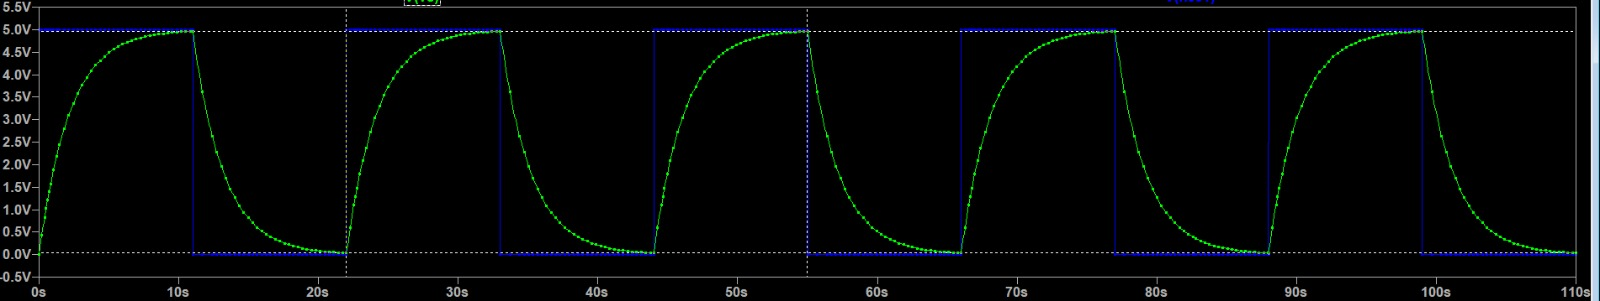
\includegraphics[width=\linewidth]{figs/lt2.jpeg}
\end{figure}
From the figure we can clearly see that the simulation matches the figure that we obtained on the CRO 
\begin{figure}[H]
    \centering
    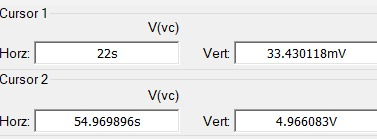
\includegraphics[width=0.5\linewidth]{figs/lt2.1.jpeg}
\end{figure}
On placing cursors at the crest and trough, we get the following values
\begin{itemize}
    \item $V_{max}=4.9660$
    \item $V_{min} = 33 mV$
\end{itemize}
The values match approximately with the ones on the CRO, hence the plot is verified 
\subsubsection{Verification using python}
It is difficult to prove the steady state values mathematically hence we use python. Below are code snippets that help verify the steady state value \\
The input variables for the code are given below 
\begin{lstlisting}[language=python]
V_high = 5          # High voltage of the square wave (V)
V_low = 0           # Low voltage of the square wave (V)
T = 22               # Time period of the square wave (s)
RC = 2.2            # RC time constant (s)
duty_cycle = 0.5    # Duty cycle (50%)
t_high = duty_cycle * T  # Time duration of high phase
t_low = (1 - duty_cycle) * T  # Time duration of low phase
\end{lstlisting}
The below snippet iteratively calculates the steady-state response of an RC circuit under a square wave input
\begin{lstlisting}[language=python]
while True:
    # Calculate new crest voltage during charging
    V_crest_new = V_high + (V_trough_prev - V_high) * np.exp(-t_high / RC)
    
    # Calculate new trough voltage during discharging
    V_trough_new = V_low + (V_crest_new - V_low) * np.exp(-t_low / RC)
    
    # Check for convergence
    if abs(V_crest_new - V_crest_prev) < tolerance and abs(V_trough_new - V_trough_prev) < tolerance:
        break
    
    # Update previous values for the next iteration
    V_crest_prev = V_crest_new
    V_trough_prev = V_trough_new
\end{lstlisting}
On executing this python code we get the values of $V_{max} = 4.966536$ and $V_{min} = 0.033464$ \\
Which is close to the values obtained on simulation via LTspice and the CRO \\
Hence the steady state response for $RC\ll T$ is verified 
\subsubsection{Single Waveform}
The single waveform obtained for 5 cycles is below 
\begin{figure}[H]
    \centering
    \includegraphics[width=0.7\linewidth]{figs/t>>RC-s.jpeg}
\end{figure}
The transient response is obtained for the below parameters, no. of cycles is set to 5. But the no of cycles visible are only 3, set the zoom to low to see all the 5 cycles 
\begin{figure}[H]
    \centering
    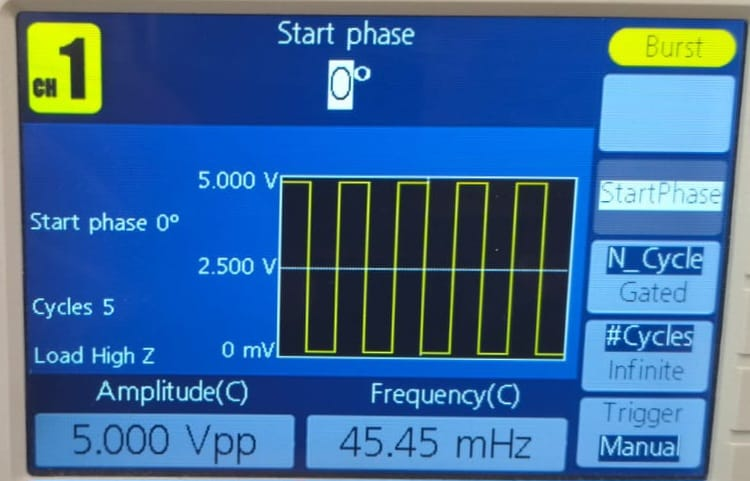
\includegraphics[width=0.5\linewidth]{figs/ip2.jpeg}
\end{figure}
\subsubsection{Mathematical Proof}

For this case, \( t \gg RC \), meaning the time constant is much smaller than the period of the square wave, so the capacitor will have enough time to charge and discharge during the input's cycle.

During the charging phase, the voltage across the capacitor increases according to the equation:

\[
V_c(t) = V_{\text{max}} \left( 1 - e^{-\frac{t}{\tau}} \right)
\]

Where:
- \( V_c(t) \) is the voltage across the capacitor at time \( t \),
- \( V_{\text{max}} = 5.041 \, \text{V} \) is the maximum voltage across the capacitor,
- \( \tau = 2.2 \, \text{s} \) is the time constant,
- \( t \) is the time elapsed during the charging phase.

During the Charging Phase: \\ 

At the beginning of the charging phase, \( t = 0 \), and the capacitor voltage is zero. As time passes, the capacitor charges according to the exponential equation.

For instance, after one time constant (\( t = \tau \)):

\[
V_c(\tau) = 5.041 \left( 1 - e^{-1} \right) = 5.041 \left( 1 - 0.3679 \right) = 5.041 \times 0.6321 = 3.18 \, \text{V}
\]

After two time constants (\( t = 2\tau \)):

\[
V_c(2\tau) = 5.041 \left( 1 - e^{-2} \right) = 5.041 \left( 1 - 0.1353 \right) = 5.041 \times 0.8647 = 4.36 \, \text{V}
\]

As the charging phase continues, the capacitor voltage approaches the maximum voltage \( V_{\text{max}} = 5.041 \, \text{V} \).

During the Discharging Phase: \\ 

During the discharging phase, the voltage across the capacitor decreases exponentially according to the equation:

\[
V_c(t) = V_{\text{initial}} e^{-\frac{t}{\tau}}
\]

Where:
- \( V_{\text{initial}} \) is the voltage across the capacitor at the start of the discharging phase.

For example, if the capacitor is charged to \( 5 \, \text{V} \) at the end of the charging phase, the voltage across the capacitor at the end of one time constant during discharging is:

\[
V_c(\tau) = 5 \times e^{-1} = 5 \times 0.3679 = 1.84 \, \text{V}
\]
Time for the Voltage to Change: \\

The time required for the capacitor to charge up to a certain voltage \( V_c \) during the charging phase is given by:

\[
t = -\tau \ln \left( 1 - \frac{V_c}{V_{\text{max}}} \right)
\]

Substituting \( V_c = 5.041 \, \text{V} \), the voltage across the capacitor reaches its maximum value after a significant period of charging.

Since \( t \gg RC \), the capacitor will charge and discharge in each cycle, with the voltage staying within a range close to \( 5.041 \, \text{V} \) (maximum) and \( 0 \, \text{V} \) (minimum) after many cycles.

The voltage across the capacitor after a time \( T/2 = 11 \, \text{s} \) during the charging phase is approximately:

\[
V_c(11 \, \text{s}) = 5.041 \left( 1 - e^{-\frac{11}{2.2}} \right)
\]
\[
V_c(11 \, \text{s}) = 5.041 \left( 1 - e^{-5} \right)
\]
\[
V_c(11 \, \text{s}) \approx 5.041 \times (1 - 0.0067) = 5.041 \times 0.9933 = 5.009 \, \text{V}
\]

Thus, the voltage at \( T/2 \) is approximately \( 5.009 \, \text{V} \), which is very close to the maximum voltage. \\ 
Hence the values for $RC\ll T$ are verified both mathematically and via simulation 

\section{Case III : $RC \gg T$}
In this case the time constant $RC$ is much greater than  the time period of the curve 
\subsection{Diagram}
\begin{center}
    \begin{figure}[!ht]
\centering
\resizebox{0.6\textwidth}{!}{% Adjusted size to fit better
\begin{circuitikz}
\tikzstyle{every node}=[font=\small]

% Main circuit connections
\draw (5,11.5) to[short] (5,9.75); % Vertical connection
\draw (5,11.5) to[short] (7.25,11.5); % Horizontal connection
\draw (7.25,11.5) to[R] (9.25,11.5); % Resistor
\draw (9.25,11.5) to[short] (9.25,10.5); % Vertical to capacitor
\draw (9.25,10.5) to[C] (9.25,8.75); % Capacitor
\draw (5,9.75) to[square voltage source] (5,8); % Voltage source
\draw (5,8) to[short] (9.25,8); % Bottom horizontal connection
\draw (9.25,8.75) to[short] (9.25,8); % Short to ground

% Labels
\node [font=\small] at (4.25,9) {5V}; % Voltage source label
\node [font=\small] at (8.25,12.25) {10k$\ohm$}; % Resistor label
\node [font=\small] at (10.25,9.5) {220$\mu$F}; % Capacitor label

% Output and arrows
\draw (9.25,11.5) to[short] (12.5,11.5); % Horizontal connection from resistor
\draw (9.25,8) to[short] (12.5,8); % Horizontal connection from ground
\node [font=\large] at (12.5,9.5) {V$_c$}; % Label for capacitor voltage
\draw [->, >=Stealth] (12.5,9.75) -- (12.5,11.5); % Arrow to top
\draw [->, >=Stealth] (12.5,9.25) -- (12.5,8); % Arrow to bottom

% Ground symbol
\draw (9.25,8) to (9.25,7.25) node[ground] {}; % Ground connection

% Input voltage label
\node [font=\large] at (5.75,8.75) {V$_{\text{in}}$}; % Label for input voltage

\end{circuitikz}
}%
\end{figure}
\end{center}
\subsection{Input signal}
The input signal is a square wave with a time period \( T = 0.22 \, \text{s} \), alternating between +5V and -5V. 
\begin{figure}[ht]
    \centering
    \begin{tikzpicture}
        \begin{axis}[
            width=10cm, height=6cm,
            grid=major,
            grid style={dashed, gray!30},
            axis lines=middle,
            xlabel={Time (s)},
            ylabel={Voltage (V)},
            xmin=0, xmax=0.88,
            ymin=-5.5, ymax=5.5,
            xtick={0,0.2,0.4,0.6,0.8},
            ytick={-5, -4, -3, -2, -1, 0, 1, 2, 3, 4, 5},
            every axis x label/.style={at={(current axis.right of origin)}, anchor=north, yshift=-15pt},
            every axis y label/.style={at={(current axis.above origin)}, anchor=east, xshift=-5pt},
            legend pos=south east,
            legend style={draw=none, fill=white, font=\small}
        ]
            % Square wave plot for period 0.22 s
            \addplot[blue, thick] coordinates {
                (0,5) (0.11,5) (0.11,-5) (0.22,-5)
                (0.22,5) (0.33,5) (0.33,-5) (0.44,-5)
                (0.44,5) (0.55,5) (0.55,-5) (0.66,-5)
                (0.66,5) (0.77,5) (0.77,-5) (0.88,-5)
            };
        \end{axis}
    \end{tikzpicture}
\end{figure}

\subsection{Input parameters}
\begin{itemize}
    \item $R$ = $10 k \ohm$
    \item $C$ = $220 \mu F$
    \item Square wave input 
        \begin{itemize}
            \item Amplitude = $\pm 5$
            \item Frequency = $454545$Hz
            \item Time Period = $0.22s$
        \end{itemize}
\end{itemize}
The value of the time constant in our experiment is $10\times 10^3 \times220 
 \times 10^{-6}$ = $2.2$
\subsection{Observations}
\begin{itemize}
    \item Connect all the components according to the circuit diagram 
    \item Input the signals and parameters mentioned above
    \item First we get a \textbf{periodic(continuous)waveform} and then we fix the number of cycles to get a \textbf{single(captured) waveform}  
\end{itemize}

\subsubsection{Continuous Waveform}
\begin{figure}[H]
    \centering
    \includegraphics[width=0.75\linewidth]{figs/T<<rc.jpeg}
\end{figure}
\begin{table}[h]
    \centering
    \renewcommand{\arraystretch}{1.3} % Adjust row height for better readability
    \begin{tabular}{|l|c|}
        \hline
        \textbf{Parameter} & \textbf{Value} \\
        \hline
        Waveform Type & Square Wave \\
        \hline
        Period & 0.220 s \\
        \hline
        Frequency & $\frac{1}{0.22} = 4.5454$ Hz \\
        \hline
        High Level Voltage & 5.000 V \\
        \hline
        Low Level Voltage & 0 mV (0 V) \\
        \hline
        Start Phase & 0° \\
        \hline
    \end{tabular}
\end{table}
The above table are the set of values inputted on the function generator
\subsubsection{Plotting using LTspice}
On simulating the below circuit on LTspice with $T=0.22$s, we can verify the figure that we obtained on the CRO for steady state response 
\begin{center}
    \begin{circuitikz}
\tikzstyle{every node}=[font=\normalsize]
\draw (3.5,10.5) to[short] (3.5,8.25);
\draw (3.5,8.25) to[square voltage source, sources/symbol/rotate=auto] (3.5,7);
\draw (3.5,10.5) to[short] (5,10.5);
\draw (5,10.5) to[R,l={ \normalsize 10k}] (7.75,10.5);
\draw (7.75,10.5) to[C,l={ \normalsize 200$\mu$}] (7.75,6.75);
\draw (3.5,7) to[short] (3.5,6.5);
\draw (3.5,6.5) to[short] (5.5,6.5);
\draw (5.5,6.5) to[short] (7.75,6.5);
\draw (7.75,6.75) to[short] (7.75,7.75);
\draw (7.75,7.75) to[short] (7.75,6.5);
\node [font=\normalsize] at (8,10.75) {$V_c$};
\node [font=\normalsize] at (6.25,10) {$R_1$};
\node [font=\normalsize] at (7,8.75) {$C_1$};
\node [font=\normalsize] at (2.75,7.75) {$V_{in}$};
\end{circuitikz}
\end{center}
\begin{figure}[H]
    \centering
    \includegraphics[width=\linewidth]{figs/t<<Rc-c.jpeg}
\end{figure}
\begin{figure}[H]
    \centering
    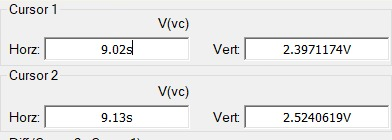
\includegraphics[width=0.5\linewidth]{figs/lt3.jpeg}
\end{figure}

The steady state values obtained on simulation are  
\begin{itemize}
    \item $V_{max} = 2.5240619V$
    \item $V_{min} = 2.3971174 V$
\end{itemize}
The values match approximately with the ones on the CRO, hence the plot is verified by simulation 
\subsubsection{Verification using Python}
It is difficult to prove the steady state values mathematically hence we use python. Below are code snippets that help verify the steady state value \\
The input variables for the code are given below
\begin{lstlisting}[language=python]
V_high = 5          # High voltage of the square wave (V)
V_low = 0           # Low voltage of the square wave (V)
T = 0.22               # Time period of the square wave (s)
RC = 2.2            # RC time constant (s)
duty_cycle = 0.5    # Duty cycle (50%)
t_high = duty_cycle * T  # Time duration of high phase
t_low = (1 - duty_cycle) * T  # Time duration of low phase
\end{lstlisting}
The below snippet iteratively calculates the steady-state crest and trough voltages of an RC circuit under a square wave input
\begin{lstlisting}[language=python]
while True:
    # Calculate new crest voltage during charging
    V_crest_new = V_high + (V_trough_prev - V_high) * np.exp(-t_high / RC)
    
    # Calculate new trough voltage during discharging
    V_trough_new = V_low + (V_crest_new - V_low) * np.exp(-t_low / RC)
    
    # Check for convergence
    if abs(V_crest_new - V_crest_prev) < tolerance and abs(V_trough_new - V_trough_prev) < tolerance:
        break
    
    # Update previous values for the next iteration
    V_crest_prev = V_crest_new
    V_trough_prev = V_trough_new
\end{lstlisting}
On executing this python code we get the values of $V_{max} = 2.562478$ and $V_{min} = 2.437505$ \\
Which are close to the values obtained on simulation via simulation and the CRO \\
Hence the steady state response for $RC \gg T$ is verified 

\subsubsection{Single Waveform}
The single waveform obtained for 6 cycles is below 
\begin{figure}[H]
    \centering
    \includegraphics[width=0.8\linewidth]{figs/t<<RC-s.jpeg}
\end{figure}
The transient response is obtained for the below parameters, no. of cycles is set to 6
\begin{figure}[H]
    \centering
    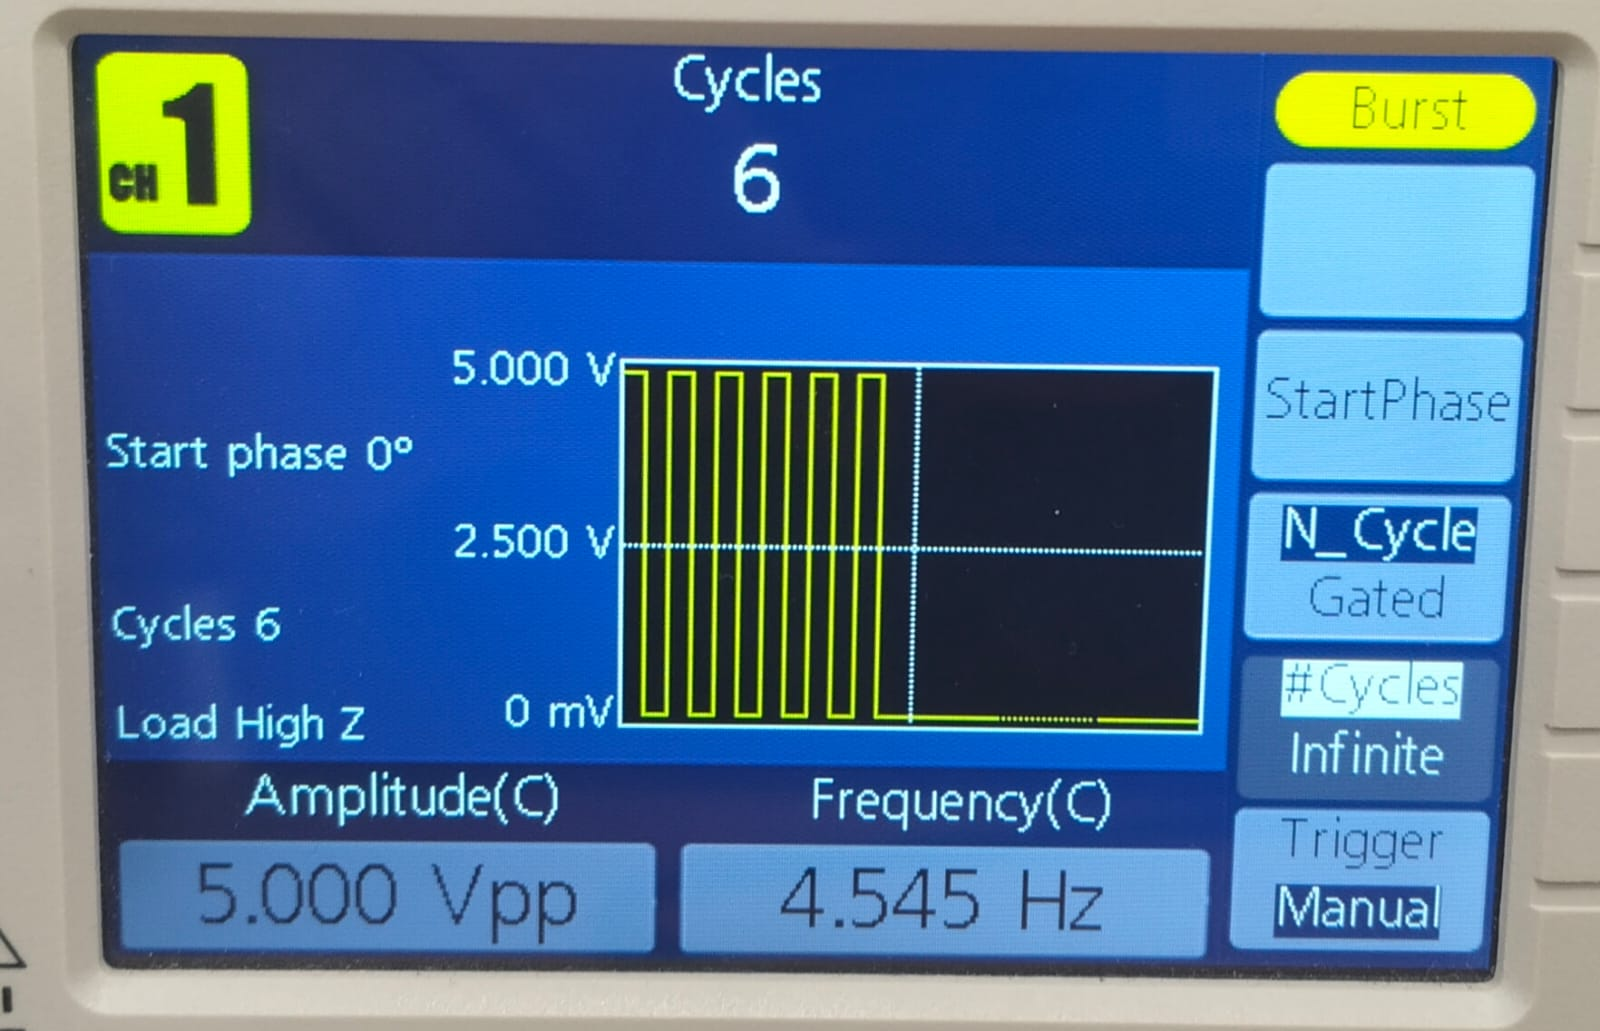
\includegraphics[width=0.5\linewidth]{figs/3-cycles.jpeg}
\end{figure}
\subsubsection{Mathematical Proof}

During the charging of the capacitor, the voltage across it is given by:
\begin{align*}
    V_c = V_{max}\left(1 - e^{\frac{-t}{\tau}}\right)
\end{align*}
where $t$ goes from $0$ to $\frac{T}{2}$.

During the discharging phase, the voltage follows:
\begin{align*}
    V_c = V_{initial} e^{\frac{-t}{\tau}}
\end{align*}
where $V_{initial}$ is the voltage at $t = \frac{T}{2}$.\\

\textbf{Given values:}
- $\tau = 2.2s$ (RC time constant)
- $T = 0.22s$ (Time period)
- $\frac{T}{2} = 0.11s$
- $V_{max} \approx 2.641V$

\textbf{Step 1: Calculating $V_c(\frac{T}{2})$ (Voltage at half-period during charging)}
\begin{align*}
    V_c(\frac{T}{2}) &= V_{max}\left(1 - e^{-\frac{T/2}{\tau}}\right) \\
    &= 2.641 \left(1 - e^{-\frac{0.11}{2.2}}\right) \\
    &= 2.641 \left(1 - e^{-0.05}\right)
\end{align*}
Using $e^{-0.05} \approx 0.9512$:
\begin{align*}
    V_c(\frac{T}{2}) &= 2.641 \times (1 - 0.9512) \\
    &= 2.641 \times 0.0488 \\
    &\approx 0.129V
\end{align*}

\textbf{Step 2: Calculating $V_C(T)$ (Voltage at full period during discharging)}
\begin{align*}
    V_C(T) &= V_{initial} e^{-\frac{T/2}{\tau}} \\
    &= 0.129 e^{-\frac{0.11}{2.2}} \\
    &= 0.129 e^{-0.05}
\end{align*}
Using $e^{-0.05} \approx 0.9512$:
\begin{align*}
    V_C(T) &= 0.129 \times 0.9512 \\
    &\approx 0.123V
\end{align*}

The values of $V_C(T)$ and $V_C(T/2)$ closely match the oscilloscope readings, confirming the transient response behavior mathematically.

\subsubsection{Plotting using LTspice}
\begin{figure}[H]
    \centering
    \includegraphics[width=\linewidth]{figs/t<<rc-s.jpeg}
\end{figure}
\begin{figure}[H]
    \centering
    
\includegraphics[width=0.7\linewidth]{figs/ip3.jpeg}
\end{figure}
The value for $V_{max}$ for transient response via simulation is 0.129 and the value for $V_{max}$ obtained on the CRO is 0.123. Since these values are approximately equal, the error might be because of noise and other practical factors.\\
Hence, the transient response for $RC >> T$ over 6 cycles is successfully verified both mathematically and through simulation.





\end{document}
